\chapter{Metodologia}
Este estudo tem como objetivo a construção de uma ontologia de domínio voltada à formalização do MPO \cite{vieira2022thesis}. O MPO configura-se como um modelo conceitual de natureza descritiva, estruturado em três dimensões principais — Estruturas, Processos e Agentes — que organizam e relacionam um conjunto de 61 conceitos distribuídos em diferentes níveis de abstração. Embora o modelo apresente consistência conceitual e relevância teórica para a estruturação de observatórios de projetos, sua representação é essencialmente textual, o que limita sua formalização.

No que se refere à sua classificação ontológica, a ontologia desenvolvida situa-se, quanto ao grau de formalismo, entre ontologias leves e ontologias pesadas, uma vez que apresenta uma estrutura conceitual rigorosa, com definições explícitas de classes, relações, propriedades e restrições, sem, contudo, empregar axiomatizações lógicas altamente expressivas ou mecanismos de raciocínio complexos. Em relação ao nível de generalidade, trata-se de uma ontologia intermediária, pois não se configura como uma ontologia de topo nem como uma ontologia de aplicação específica, atuando como elo conceitual entre uma ontologia fundamental e possíveis ontologias de aplicação no domínio de observatórios de projetos. Quanto à sua finalidade, a ontologia é classificada como uma ontologia de domínio, por formalizar conhecimentos específicos relacionados ao contexto de observatórios de projetos.

Diante desse contexto, a presente pesquisa tem caráter teórico-conceitual, com foco na engenharia do conhecimento, e busca suprir a lacuna relacionada à ausência de uma representação formal do MPO. A ontologia proposta não tem como finalidade a a sua aplicação direta em sistemas computacionais, mas sim a formalização ontológica dos conceitos, relações e restrições definidos no modelo original, de modo a torná-lo semanticamente explícito, não ambíguo e computacionalmente interpretável.

Do ponto de vista metodológico, trata-se de uma pesquisa de natureza qualitativa, fundamentada em uma abordagem interpretativista, uma vez que se dedica à análise, compreensão e explicitação de um modelo conceitual existente. A investigação baseia-se predominantemente em pesquisa documental, utilizando como fontes principais os documentos oficiais do MPO, publicações científicas correlatas e literatura especializada em ontologias e observatórios. A análise dos dados foi conduzida por meio de análise de conteúdo, com o objetivo de identificar, organizar e sistematizar os conceitos, relações e atributos relevantes ao domínio.

A condução da pesquisa foi estruturada em duas etapas principais. Na primeira, realizou-se uma revisão exploratória da literatura, com o propósito de fundamentar teoricamente os conceitos de observatórios, transparência, ontologias e metodologias de engenharia ontológica. Na segunda etapa, procedeu-se ao desenvolvimento da ontologia, denominada OntoMPO, seguindo as diretrizes da metodologia \textit{Methontology} \cite{fernandez1997methontology}.

A \textit{Methontology} define um conjunto sistemático de atividades voltadas à construção de ontologias, abrangendo atividades de gestão e de suporte que acompanham todo o ciclo de vida do artefato ontológico. Paralelamente, a metodologia estabelece seis etapas principais de desenvolvimento: especificação, conceitualização, formalização, integração, implementação e avaliação, organizadas em um ciclo contínuo de evolução do modelo. Assim, esta seção está estruturada de acordo com essas etapas, descrevendo de forma detalhada como cada uma foi aplicada no processo de construção da OntoMPO, bem como as atividades de gestão e suporte realizadas ao longo do desenvolvimento.

\begin{figure}[H]
    \centering
    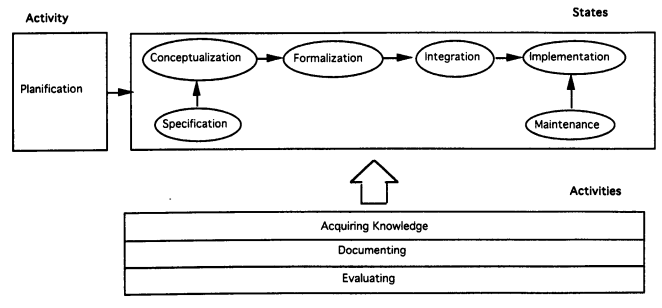
\includegraphics[width=0.8\linewidth]{imagens/methontology.png}
    \caption{\textit{Methontology}. Fonte: \citeauthor{fernandez1997methontology}}
    \label{fig:mpo_class_tree}
\end{figure}

A escolha da \textit{Methontology} como metodologia de referência justifica-se por
seu caráter consolidado e amplamente adotado na literatura de engenharia
ontológica, oferecendo um conjunto bem definido de etapas, atividades e
artefatos que orientam de forma sistemática todo o ciclo de desenvolvimento
de uma ontologia, desde a especificação até a avaliação. Essa estrutura
detalhada e a disponibilidade de artefatos intermediários bem documentados
(glossário de termos, árvore de classificação, dicionário de conceitos,
entre outros) tornam a metodologia adequada para um trabalho de mestrado
com escopo conceitual bem definido, no qual a rastreabilidade entre os
conceitos do modelo original e os elementos da ontologia resultante é um
requisito relevante.

\section{Especificação}
A etapa de especificação, conforme estabelecida pela \textit{Methontology} \cite{fernandez1997methontology}, tem como objetivo definir o escopo e os requisitos da ontologia a ser desenvolvida, identificando o domínio de interesse, os objetivos do modelo ontológico e os principais stakeholders envolvidos. Nessa etapa, são estabelecidos os limites da ontologia, bem como os requisitos informacionais que ela deve atender, servindo de base para orientar as atividades subsequentes do processo de desenvolvimento ontológico.

\subsection{Propósito da ontologia}
A ontologia proposta neste trabalho tem como finalidade representar e formalizar, de maneira conceitualmente rigorosa e semanticamente consistente, os conceitos centrais do Modelo para Observatórios de Projetos (MPO) \cite{vieira2022thesis}. Seu propósito principal é explicitar o conhecimento do domínio dos observatórios de projetos em uma estrutura formal e computacionalmente interpretável, preservando a semântica do modelo conceitual original e reduzindo ambiguidades inerentes à sua representação textual.

Ao formalizar o MPO, a ontologia possibilita a análise conceitual sistemática do modelo, a verificação de coerência lógica entre seus elementos e a explicitação das relações e dependências semânticas existentes entre conceitos, processos e agentes. Trata-se, portanto, de uma ontologia de domínio voltada à padronização conceitual e à organização semântica do MPO, concebida como um artefato fundacional que pode subsidiar estudos analíticos, extensões conceituais e futuras aplicações computacionais.

Embora a representação formal adotada permita o suporte a mecanismos computacionais, o escopo deste trabalho concentra-se na construção, documentação e avaliação estrutural da ontologia.

\subsubsection{Formalização de conceitos, relações e atributos essenciais}
Na ontologia proposta, a formalização de \textbf{conceitos, relações e atributos} consiste na tradução do conhecimento do domínio, originalmente descrito de forma conceitual e textual no MPO \cite{vieira2022thesis}, para uma representação formal baseada em ontologias. Os \textbf{conceitos} do modelo são representados como classes ontológicas, dotadas de identificadores únicos, hierarquia explicitada e definições formais, promovendo padronização terminológica e clareza semântica.

As \textbf{relações} expressam os vínculos semânticos entre os conceitos do domínio, como a associação entre processos e os conteúdos que produzem ou entre agentes e suas responsabilidades. Essas relações são formalizadas como propriedades de objeto, com definição explícita de domínio e alcance e, quando pertinente, com restrições de cardinalidade e características lógicas que tornam explícitas regras conceituais implícitas no modelo original.

Os \textbf{atributos} descrevem características literais dos conceitos, como nomes, datas, níveis ou prioridades, sendo modelados como propriedades de dados com tipos bem definidos. Essa formalização permite que a estrutura conceitual do MPO seja interpretada de maneira não ambígua por agentes humanos e computacionais, constituindo uma base formal para análises semânticas e verificações de consistência.

\subsubsection{Padronização terminológica e semântica}
Em ambientes nos quais diferentes observatórios de projetos são desenvolvidos de forma independente, é comum que conceitos semanticamente equivalentes sejam nomeados de maneiras distintas, refletindo escolhas locais, contextos organizacionais ou preferências terminológicas. Essas variações não se limitam a diferenças lexicais, mas frequentemente envolvem ambiguidades quanto ao papel, às responsabilidades e às relações associadas a cada conceito.

Por exemplo, no contexto do MPO, o conceito de entidade que interage com o observatório pode ser representado de diferentes formas:

\begin{itemize}
    \item um observatório pode utilizar o termo “usuário” para designar indivíduos que acessam informações e acompanham projetos;
    \item outro pode empregar a denominação “colaborador” para representar participantes que contribuem com dados, análises ou avaliações;
    \item um terceiro pode adotar o termo “agente” para abranger, de forma mais ampla, tanto participantes humanos quanto sistemas externos que interagem com o observatório.
\end{itemize}

Na ausência de uma formalização ontológica, essas denominações tendem a ser tratadas como conceitos distintos, dificultando a comparação conceitual, a integração de informações e a interoperabilidade semântica entre observatórios. Com a adoção da ontologia, esses diferentes termos podem ser mapeados para uma classe ontológica comum, como \texttt{mpo:Agent}, cuja definição formal explicita suas características essenciais, suas possíveis especializações e suas relações com outros elementos do domínio, como processos, estruturas e conteúdos.

Dessa forma, a ontologia não apenas uniformiza a terminologia, mas também estabelece um entendimento semântico compartilhado sobre o papel e o significado do conceito no contexto do MPO. Esse mecanismo favorece a padronização conceitual do domínio e cria condições para futuras integrações semânticas, permitindo que consultas, análises e comparações conceituais sejam formuladas de maneira consistente, independentemente da nomenclatura originalmente adotada por cada observatório.

\subsubsection{Usuários alvo}
\begin{itemize}
    \item Equipes que desenvolvem observatórios de projetos baseados no MPO\cite{vieira2022thesis}: Grupos responsáveis pelo planejamento, implementação e manutenção de observatórios que adotam o Modelo para Observatório de Projetos como referência conceitual. Essas equipes podem utilizar a ontologia para padronizar a modelagem de dados, garantir consistência terminológica entre módulos e sistemas, facilitar a integração de fontes de informação heterogêneas e possibilitar consultas semânticas avançadas. A aplicação da ontologia nesse contexto também apoia a replicação de boas práticas em diferentes instâncias do MPO\cite{vieira2022thesis}, assegurando que novas implementações mantenham compatibilidade e interoperabilidade com soluções já existentes;
    \item Pesquisadores e acadêmicos: Profissionais e estudantes interessados em ontologias, que podem utilizar esta como referência para desenvolver seus próprios modelos seguindo as etapas apresentadas neste estudo. Além de servir como guia metodológico, a ontologia funciona como exemplo prático de construção baseada em modelos conceituais já existentes, permitindo compreender como transformar representações teóricas em estruturas formais reutilizáveis;
\end{itemize}

\subsection{Nível de formalidade}
A ontologia desenvolvida neste trabalho é construída de forma progressiva, evoluindo de um nível semi-formal para um nível formal, em conformidade com as diretrizes da metodologia \textit{Methontology}. Inicialmente, o domínio é representado em nível semi-formal por meio de diagramas conceituais, taxonomias e descrições textuais estruturadas, utilizadas para explicitar conceitos, relações e atributos do MPO e apoiar a compreensão e validação conceitual do modelo.

Na etapa de formalização e implementação, a ontologia é expressa em um nível formal, por meio da linguagem OWL 2 DL, assegurando uma representação computacional precisa e semanticamente rigorosa. A escolha dessa linguagem permite a definição explícita de classes, propriedades, restrições e axiomas, bem como a verificação automática de coerência e consistência lógica por meio de motores de raciocínio compatíveis.

A implementação da ontologia é realizada com o apoio de ferramentas adequadas à engenharia ontológica, possibilitando sua codificação, edição e avaliação estrutural. O uso dessas ferramentas visa garantir que a ontologia seja interpretável tanto por especialistas humanos quanto por sistemas computacionais, restringindo-se, no escopo deste trabalho, à validação lógica, à análise conceitual e à documentação formal do modelo ontológico, sem contemplar sua aplicação em cenários operacionais ou o uso extensivo de instâncias e consultas semânticas.

\subsection{Escopo}
A ontologia proposta abrange integralmente as três camadas do MPO\cite{vieira2022thesis}, que são \textbf{Estruturas}, \textbf{Processos} e \textbf{Agentes}, garantindo a representação formal de seus conceitos gerais, intermediários e específicos. Na camada \textbf{Estruturas} serão modelados os elementos que compõem a organização e a infraestrutura de um observatório. Na camada \textbf{Processos} a ontologia contemplará atividades e fluxos de trabalho que sustentam o funcionamento do observatório. Na camada \textbf{Agentes} serão representados os atores que interagem com o observatório, suas funções e papéis, bem como suas motivações e vínculos com processos e estruturas. A modelagem incluirá propriedades de objeto para estabelecer as relações entre os conceitos das diferentes camadas, por exemplo, Processo produz Conteúdo, Agente executa Processo e Estrutura suporta Processo. Também serão definidas propriedades de dados para descrever atributos relevantes. O nível de granularidade adotado permitirá detalhar desde as classes mais gerais até os conceitos específicos, preservando a coerência conceitual.

\subsection{Fontes de conhecimento}
\begin{enumerate}
    \item Observatórios de Projetos: Um Modelo Conceitual\cite{vieira2022thesis};
\end{enumerate}

\subsection{Questões de competência}
As questões de competência definem o conjunto mínimo de perguntas que a ontologia deve ser capaz de responder, orientando sua modelagem e servindo como critério de avaliação de sua adequação ao domínio do MPO.

\begin{enumerate}
    \item Como os conceitos estão organizados hierarquicamente dentro de cada dimensão do MPO?
    \item Como a camada de estruturas é representada?
    \item Como a camada de processos é representada?
    \item Como a camada de agentes é representada?
    \item Quais são as relações existentes entre estruturas, processos e agentes?
\end{enumerate}

\section{Conceitualização}
A etapa de conceitualização, conforme estabelecida pela \textit{Methontology} \cite{fernandez1997methontology}, tem como objetivo estruturar o conhecimento do domínio de forma independente de qualquer linguagem de implementação, organizando os conceitos, relações e atributos identificados na etapa de especificação. Nessa fase, o conhecimento do domínio é modelado em um nível conceitual, permitindo uma representação clara e compartilhável, que servirá como base para as etapas de formalização, integração e implementação da ontologia.

O modelo conceitual é expresso por meio de um conjunto de \textbf{entregáveis}, que permitem aos usuários finais:
(a) verificar se uma ontologia é útil e aplicável a uma determinada aplicação, sem a necessidade de inspecionar seu código-fonte;
(b) comparar o escopo e a completude de diferentes ontologias, bem como avaliar sua reutilização e compartilhamento, a partir da análise do conhecimento representado em cada uma das suas representações.

Os \textbf{entregáveis} dessa fase incluem um conjunto de artefatos que estruturam e formalizam o conhecimento do domínio, sendo eles:
\begin{enumerate}
    \item \textbf{Glossário de termos}: Identifica e reúne todos os recursos úteis e potencialmente utilizáveis no conhecimento do domínio e seus significados;
    \item \textbf{Árvore de classificação de conceitos}: Organizam conceitos de domínio em taxonomias. Eles são usados não apenas para saber como os conceitos se relacionam, mas para modularizar o conhecimento do domínio;
    \item \textbf{Diagrama de verbos}: Expressar o significado dos verbos de forma declarativa;
    \item \textbf{Tabela de fórmulas}: Formaliza as restrições e relações estáticas da ontologia, ou seja, axiomas e invariantes sobre os conceitos, atributos e relacionamentos.;
    \item \textbf{Tabela de regras}: Lista as regras deriváveis que expressam comportamentos dinâmicos, inferências ou efeitos das ações;
\end{enumerate}

\begin{figure}[H]
    \centering
    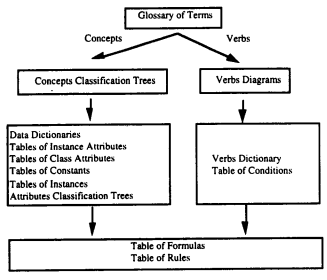
\includegraphics[width=0.6\linewidth]{imagens/methontology_conceptualization.png}
    \caption{Etapa de conceitualização da \textit{Methontology}. Fonte: \citeauthor{fernandez1997methontology}}
    \label{fig:mpo_class_tree}
\end{figure}

\section{Formalização}
A etapa de formalização, conforme estabelecido pela Methontology \cite{fernandez1997methontology}, tem como finalidade transformar o modelo conceitual elaborado na fase de conceitualização em uma representação formal e não ambígua. Nessa fase, o conhecimento do domínio, previamente estruturado em conceitos, relações e atributos, é expresso por meio de uma linguagem formal que possibilita sua interpretação de forma precisa por humanos e sistemas computacionais.

No contexto desta pesquisa, a formalização da ontologia foi realizada utilizando a OntoUML \cite{ontouml_readthedocs}, uma linguagem ontológica derivada da UML e fundamentada na UFO \cite{guizzardi2008grounding}. A escolha dessa linguagem se justifica pela sua capacidade de representar de maneira rigorosa e semântica os elementos conceituais identificados, possibilitando uma correspondência fiel entre os constructos do MPO\cite{vieira2022thesis} e os elementos ontológicos formais.

Durante o processo de formalização, os conceitos das dimensões Estruturas, Processos e Agentes foram modelados como classes ontológicas, seguindo as categorias ontológicas propostas pela UFO, tais como \textit{Kind}, \textit{Role}, \textit{Relator} e \textit{Mode}. As relações entre os conceitos (por exemplo, executa, gera, apoia, pertence a) foram formalizadas como associações ontológicas, especificando seus domínios, alcances, multiplicidades e restrições. Já os atributos foram descritos como propriedades intrínsecas ou relacionais, garantindo coerência com as categorias ontológicas associadas a cada classe.

A consistência semântica e ontológica do modelo foi assegurada mediante validação manual, com base nas regras de modelagem da OntoUML e nas categorias ontológicas da UFO, garantindo fidelidade conceitual ao domínio do MPO. Dessa forma, a formalização desempenha o papel de ponte entre a representação conceitual e sua execução prática, garantindo que a ontologia resultante seja semanticamente coerente, formalmente estruturada e reutilizável em sistemas de apoio à gestão e observação de projetos.

Cabe destacar que, embora a \textit{Methontology} apresente as atividades de integração e formalização como etapas distintas, neste trabalho essas atividades foram conduzidas de forma iterativa e parcialmente paralela. A integração com o MPO e com a UFO influenciou diretamente as decisões de formalização, especialmente no que se refere à classificação ontológica dos conceitos e à definição de relações e restrições. Da mesma forma, o processo de formalização em OntoUML contribuiu para o refinamento dos conceitos integrados, permitindo a identificação de ajustes semânticos e estruturais ao longo do desenvolvimento da ontologia. Essa abordagem iterativa está em conformidade com o caráter incremental da \textit{Methontology} e contribui para a construção de um modelo ontológico mais consistente e alinhado ao domínio.

A flexibilização na execução sequencial dessas etapas não comprometeu a
rastreabilidade nem o rigor metodológico do processo, uma vez que os
artefatos prescritos pela Methontology \cite{fernandez1997methontology} para cada atividade --- glossário
de termos, dicionário de conceitos, tabelas de relações, atributos e
axiomas --- foram mantidos e atualizados de forma consistente a cada
ciclo de refinamento. Dessa forma, embora a execução das atividades de
integração e formalização tenha ocorrido de maneira não estritamente
sequencial, cada decisão de classificação ontológica ou ajuste estrutural
permanece registrada e justificável a partir dos artefatos conceituais
produzidos, preservando a rastreabilidade entre o MPO original e os
elementos formais da OntoMPO. Essa flexibilização está alinhada ao próprio
caráter iterativo previsto pela Methontology, que admite revisões e
realimentações entre etapas ao longo do ciclo de desenvolvimento, e não
constitui um desvio do rigor metodológico, mas sua aplicação adaptada às
necessidades específicas deste trabalho.

\section{Integração}
A atividade de integração, conforme definida na \textit{Methontology} \cite{fernandez1997methontology}, tem como objetivo promover o reuso sistemático de ontologias e modelos conceituais, de modo a reduzir ambiguidades semânticas, evitar redundâncias conceituais e aumentar a interoperabilidade e a qualidade do artefato ontológico desenvolvido. 

No contexto desta pesquisa, a integração com o MPO \cite{vieira2022thesis} ocorreu predominantemente nas etapas de \textit{especificação} e \textit{conceitualização}, nas quais os conceitos do domínio foram identificados, analisados e estruturados a partir do referido modelo. Dessa forma, a presente etapa de integração não tem como foco a incorporação conceitual do MPO, mas sim a consolidação ontológica dos conceitos previamente definidos. Nesse sentido, a integração considerada nesta etapa concentrou-se principalmente na:
\begin{enumerate}
    \item integração ontológica de fundamentação, por meio da utilização da UFO \cite{guizzardi2008grounding};
    \item articulação dos conceitos integrados e formalizados, garantindo coerência semântica e alinhamento ontológico.
\end{enumerate}

Como resultado dessa atividade, os conceitos previamente definidos nas etapas de especificação e conceitualização passaram a dispor de uma fundamentação ontológica explícita, permitindo sua correta classificação segundo as categorias da UFO \cite{vieira2022thesis} e assegurando coerência semântica ao modelo. Essa integração contribuiu diretamente para o processo de formalização em OntoUML \cite{ontouml_readthedocs}, uma vez que as decisões de modelagem foram orientadas por princípios ontológicos bem estabelecidos, reduzindo ambiguidades e favorecendo a consistência e a evolutividade da ontologia proposta.

\section{Implementação}
A etapa de implementação, conforme definida pela \textit{Methontology} \cite{fernandez1997methontology}, tem como objetivo materializar a ontologia formalizada em um ambiente computacional, utilizando uma linguagem e ferramentas que possibilitem sua manipulação, validação e uso em sistemas baseados em conhecimento. Nessa etapa, o modelo ontológico desenvolvido nas fases anteriores é traduzido para uma representação computacional executável, preservando sua semântica e estrutura formal.

No contexto desta pesquisa, a ontologia foi implementada utilizando o software Protégé, uma ferramenta amplamente adotada para o desenvolvimento, edição e gerenciamento de ontologias. O Protégé foi escolhido por oferecer suporte nativo a linguagens baseadas em lógica de descrição, como a OWL (\textit{Web Ontology Language}), além de disponibilizar recursos para edição gráfica, definição de axiomas e validação de consistência ontológica.

A implementação teve como ponto de partida o modelo ontológico formalizado em OntoUML \cite{ontouml_readthedocs}, previamente fundamentado na UFO \cite{guizzardi2008grounding}. Esse modelo foi traduzido para OWL no ambiente do Protégé, respeitando as decisões ontológicas estabelecidas na fase de formalização. As classes ontológicas foram implementadas como classes OWL, as relações foram representadas por meio de propriedades de objeto, e os atributos foram modelados como propriedades de dados, com seus respectivos domínios, alcances e restrições.

\section{Avaliação}

A etapa de avaliação, conforme estabelecido pela \textit{Methontology} \cite{fernandez1997methontology}, tem como objetivo verificar a qualidade da ontologia desenvolvida, assegurando que ela atenda aos requisitos definidos na etapa de especificação e que esteja semanticamente coerente, consistente e adequada ao domínio ao qual se propõe. Diferentemente das etapas de formalização e implementação, a avaliação concentra-se na análise crítica do artefato ontológico resultante, e não em seu processo de construção.

No contexto desta pesquisa, a avaliação da ontologia foi conduzida considerando aspectos conceituais, semânticos, estruturais e funcionais, tendo como referência o MPO \cite{vieira2022thesis} e os princípios ontológicos da UFO \cite{guizzardi2008grounding}. Essa abordagem permitiu analisar se os conceitos, relações e restrições definidos refletem adequadamente o conhecimento do domínio e se estão corretamente fundamentados ontologicamente.

Inicialmente, foi realizada uma avaliação conceitual e ontológica por meio de inspeção manual do modelo, com base nas diretrizes de modelagem da OntoUML \cite{ontouml_readthedocs} e nas categorias ontológicas da UFO \cite{guizzardi2008grounding}. Essa análise teve como objetivo verificar a correta classificação dos conceitos, a coerência das hierarquias taxonômicas, a adequação das relações estabelecidas entre as dimensões do MPO (Estruturas, Processos e Agentes), bem como a ausência de ambiguidades ou contradições conceituais, assegurando fidelidade semântica ao domínio.

A avaliação funcional da ontologia foi conduzida com base em um conjunto estruturado de Questões de Competência, definidas e refinadas a partir das dimensões do MPO. Essas questões foram organizadas de modo a abranger diferentes aspectos do domínio, incluindo: (i) a estrutura conceitual do observatório, (ii) as relações entre Estruturas, Processos, Agentes e Conteúdos, (iii) os papéis desempenhados pelos agentes, (iv) os processos e seus fluxos de informação, e (v) os elementos estruturais e informacionais envolvidos.

Para verificar se a ontologia é capaz de responder às questões de competência propostas, foram utilizadas consultas em linguagem SPARQL (\textit{SPARQL Protocol and RDF Query Language}), padrão recomendado pelo W3C para consulta de dados representados em RDF \cite{sparql2013}. SPARQL permite recuperar e manipular dados estruturados em grafos RDF por meio da especificação de padrões de triplas, que correspondem à estrutura fundamental do modelo RDF, composta por sujeito, predicado e objeto.

Uma consulta SPARQL é composta, em geral, por cláusulas que definem o tipo de operação desejada e os padrões de busca no grafo RDF. Entre os elementos mais utilizados estão:

\begin{itemize}
\item \textbf{SELECT}: especifica as variáveis cujos valores devem ser retornados pela consulta;
\item \textbf{WHERE}: define o conjunto de padrões de triplas que devem ser satisfeitos no grafo RDF;
\item \textbf{PREFIX}: permite definir abreviações para namespaces utilizados na ontologia;
\item \textbf{FILTER}: possibilita aplicar restrições lógicas ou condicionais aos resultados da consulta.
\end{itemize}

Por exemplo, uma consulta SPARQL pode recuperar relações hierárquicas entre classes de uma ontologia utilizando a propriedade \textit{rdfs:subClassOf}, que representa relações de especialização entre conceitos. De forma semelhante, propriedades do tipo \textit{owl:ObjectProperty} podem ser utilizadas para identificar relações semânticas entre classes, considerando seus domínios (\textit{rdfs:domain}) e alcances (\textit{rdfs:range}).

No contexto deste trabalho, as consultas SPARQL foram utilizadas para extrair informações estruturais e semânticas da ontologia implementada em OWL, permitindo verificar aspectos como a organização hierárquica das classes e as relações existentes entre diferentes conceitos do modelo. Essas consultas foram executadas sobre a ontologia utilizando ferramentas compatíveis com o padrão RDF, permitindo acessar diretamente as triplas que compõem o grafo ontológico.

A validação consistiu na análise dos resultados retornados pelas consultas, observando se estes correspondem às respostas esperadas de acordo com o domínio do MPO. Esse procedimento permitiu avaliar a adequação da ontologia quanto à sua capacidade de suportar consultas e atender aos requisitos informacionais definidos na etapa de especificação.

Por fim, a ontologia foi avaliada segundo critérios gerais de qualidade, tais como clareza conceitual, coerência terminológica, ausência de redundâncias e potencial de reutilização e extensão. Esses critérios são fundamentais para garantir que a ontologia possa ser compreendida, mantida e aplicada em diferentes contextos, incluindo sistemas de apoio à gestão e observação de projetos.

Dessa forma, a etapa de avaliação assegura que a ontologia proposta seja conceitualmente consistente, semanticamente adequada e funcionalmente capaz de responder às questões de competência definidas, cumprindo o papel de formalização ontológica do MPO \cite{vieira2022thesis}.

\section{Manutenção}
A etapa de manutenção, conforme estabelecida pela \textit{Methontology} \cite{fernandez1997methontology}, tem como objetivo garantir a evolução controlada da ontologia ao longo do tempo, assegurando que ela permaneça consistente, atualizada e alinhada às mudanças no domínio ao qual se aplica. Essa etapa contempla a identificação, análise e incorporação de modificações necessárias, bem como a correção de eventuais inconsistências ou lacunas identificadas após a implementação e avaliação da ontologia.

No contexto desta pesquisa, a manutenção da ontologia foi concebida como um processo contínuo e incremental, a ser realizado a partir da utilização e análise da ontologia em cenários reais ou futuros do MPO \cite{vieira2022thesis}. Alterações no domínio, como a introdução de novos tipos de projetos, agentes, processos ou indicadores, podem demandar a inclusão ou refinamento de conceitos, relações e restrições ontológicas.

As atividades de manutenção incluem, entre outras, a revisão periódica das classes e propriedades existentes, a avaliação do impacto de alterações propostas sobre a estrutura ontológica e a verificação da preservação da coerência semântica e ontológica do modelo. Sempre que necessário, tais modificações devem ser conduzidas de forma alinhada às categorias ontológicas da UFO \cite{guizzardi2008grounding} e às regras de modelagem da OntoUML \cite{ontouml_readthedocs}, preservando as decisões ontológicas fundamentais estabelecidas neste trabalho.

Dessa forma, a etapa de manutenção assegura que a ontologia proposta possa evoluir de maneira controlada e consistente, mantendo sua qualidade ontológica e seu potencial de reutilização e extensão em diferentes contextos de aplicação relacionados ao MPO.
